% base code: https://tex.stackexchange.com/questions/497859/neural-network-diagram

\documentclass[border=0.125cm]{standalone}
\usepackage{tikz}
\usetikzlibrary{positioning}
\begin{document}

\tikzset{%
  every neuron/.style={
    circle,
    draw,
    minimum size=1cm
  },
  neuron missing/.style={
    draw=none, 
    scale=4,
    text height=0.333cm,
    execute at begin node=\color{black}$\vdots$
  },
}

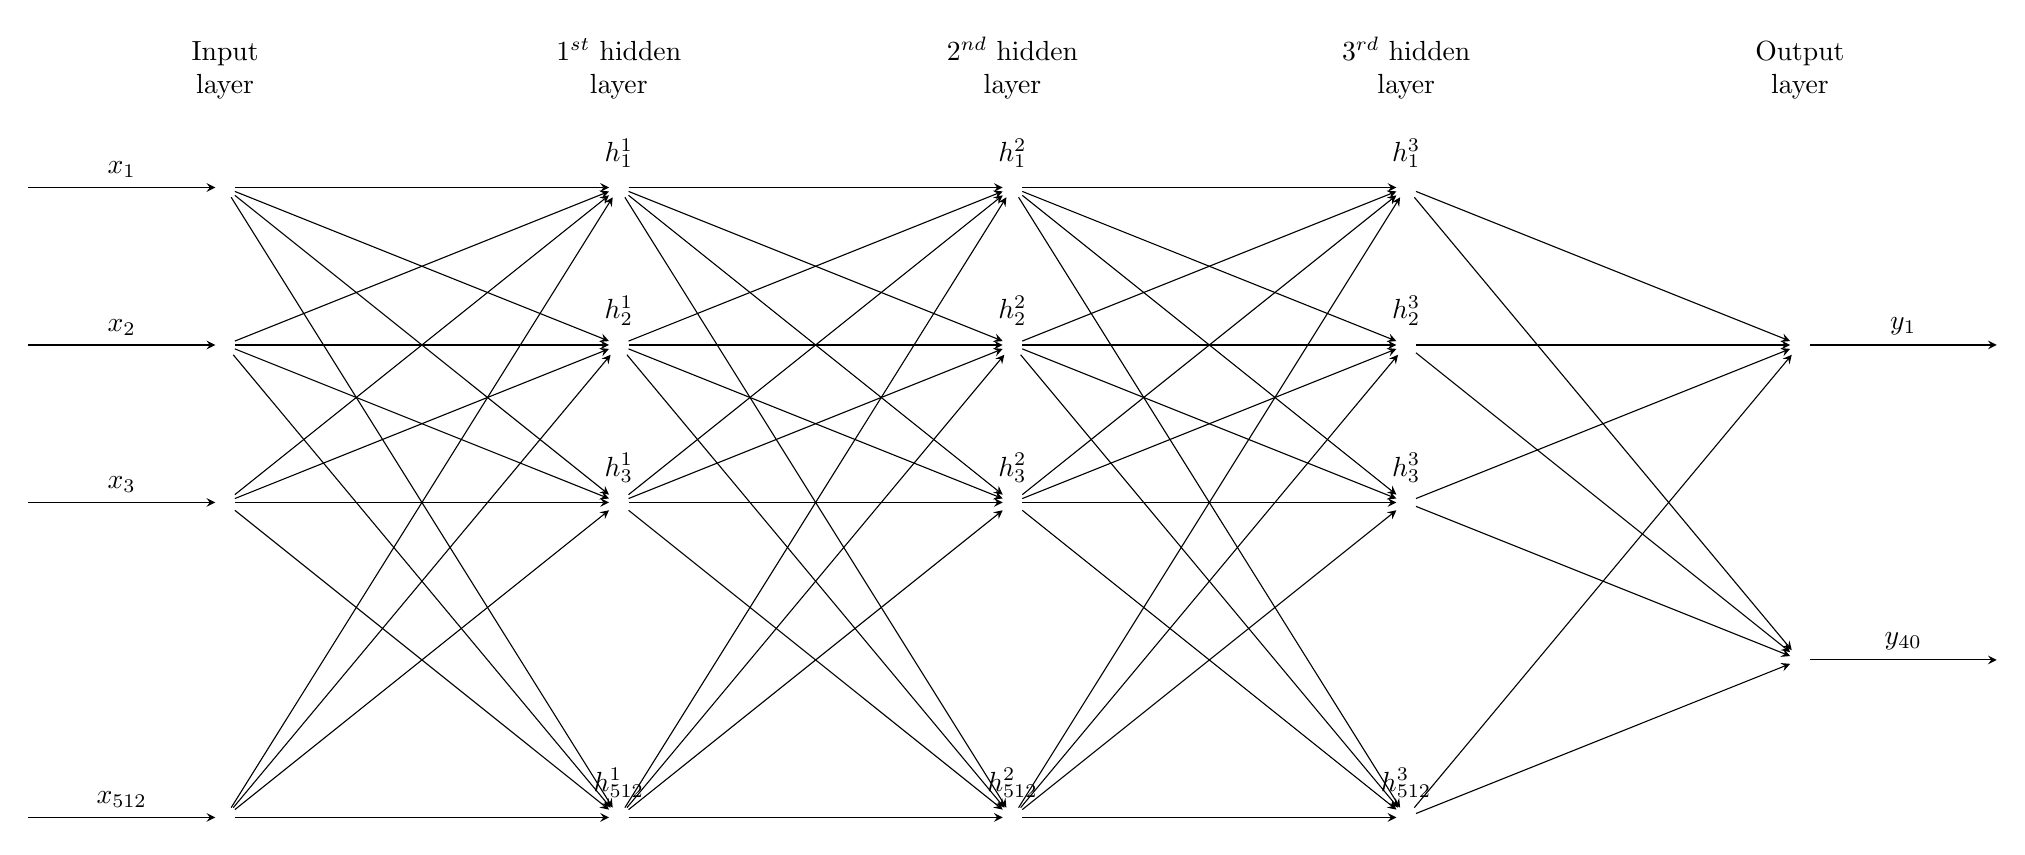
\begin{tikzpicture}[x=2.5cm, y=2cm, >=stealth]

% input
\foreach \m/\l [count=\y] in {1,2,3,missing,4}
{
  \node [every neuron/.try,neuron \m/.try] (input-\m) at (0,2.5-\y) {};
}

% h1
\foreach \m [count=\y] in {1,2,3,missing,4}
  \node [every neuron/.try, neuron \m/.try ] (hidden-\m) at (2,2.5-\y) {};
  
% h2
\foreach \m [count=\y] in {1,2,3,missing,4}
  \node [every neuron/.try, neuron \m/.try ] (h2-\m) at (4,2.5-\y) {};

% h3
\foreach \m [count=\y] in {1,2,3,missing,4}
  \node [every neuron/.try, neuron \m/.try ] (h3-\m) at (6,2.5-\y) {};

% output
\foreach \m [count=\y] in {1,missing,2}
  \node [every neuron/.try, neuron \m/.try ] (output-\m) at (8,1.5-\y) {};

% input
\foreach \l [count=\i] in {1,2,3,512}
  \draw [<-] (input-\i) -- ++(-1,0)
    node [above, midway] {$x_{\l}$};

% h1
\foreach \l [count=\i] in {1,2,3,512}
  \node [above] at (hidden-\i.north) {$h_{\l}^{1}$};

% h2
\foreach \l [count=\i] in {1,2,3,512}
  \node [above] at (h2-\i.north) {$h_{\l}^{2}$};
  
% h3
\foreach \l [count=\i] in {1,2,3,512}
  \node [above] at (h3-\i.north) {$h_{\l}^{3}$};

% output
\foreach \l [count=\i] in {1,40}
  \draw [->] (output-\i) -- ++(1,0)
    node [above, midway] {$y_{\l}$};

% Connections

% in -> h1
\foreach \i in {1,...,4}
  \foreach \j in {1,...,4}
    \draw [->] (input-\i) -- (hidden-\j);

% h1 -> h2
\foreach \i in {1,...,4}
  \foreach \j in {1,...,4}
    \draw [->] (hidden-\i) -- (h2-\j);

% h2 -> h3
\foreach \i in {1,...,4}
  \foreach \j in {1,...,4}
    \draw [->] (h2-\i) -- (h3-\j);

% h3 -> out
\foreach \i in {1,...,4}
  \foreach \j in {1,...,2}
    \draw [->] (h3-\i) -- (output-\j);

% Titles
\foreach \l [count=\x from 0] in {Input, $1^{st}$ hidden, $2^{nd}$ hidden, $3^{rd}$ hidden, Output}
  \node [align=center, above] at (\x*2,2) {\l \\ layer};

\end{tikzpicture}

\end{document}